\chapter{Reorganization of network architecture during reading and listening}

\epigraph{Reading is parasitic on language... [It] is seen not as a parallel activity in the visual mode to speech perception in the auditory mode: there are differences... [that] can be explained only if we regard reading as a deliberately acquired, language-based skill, dependent up on the speaker-hearer's awareness of certain aspects of primary linguistic activity.}{I. Mattingly, 1972 \citep{Mattingly1972}}

\section{Motivation}

In the first chapter, we established that reading utilizes a variety of cognitive skills whose neural substrates are distributed throughout the brain. But being able to comprehend speech is a pre-requisite to reading, and it is similarly complex. This begs the question: in what ways is reading unique from listening?

The most widely-held view is that reading and listening share the same core linguistic processes and differ primarily in the sensory processes that feed into supra-model linguistic systems \citep{Mattingly1972, Price2012}. One popular model, the \textit{Simple View of Reading} makes the model testable by stating that reading comprehension is the product of listening comprehension and decoding skills \citep{Gough1988}. This view has received support from large behavioral studies \citep{Kirby2006} and neuroimaging investigations: many of the literacy-related changesare linked to visual or phonological systems, areas not directly related to semantic or comprehension processes \citep{Schlaggar2006, Dahaene2015}. These findings support a model in which inputs from auditory or visual domains are fed up into higher-order association areas that sequence, encode articulatory plans, and extract semantic information \citep{Price2012}. These processes localize onto the similar areas regardless of language and writing system \citep{Rueckl2016}, and may even extend to inputs from somatosensory domains \citep{Xu2005, Sood2015}. This supra-modal language core is largely left-lateralized and centers on the inferior frontal gyrus, anterior and posterior middle temporal gyrus and the angular gyrus. Neuroanatomical models of language, shown in Fig. \ref{ch2-price-language-models}, illustrate that language is distributed throughout much of the brain. 

\begin{figure}[t]
	\centering
	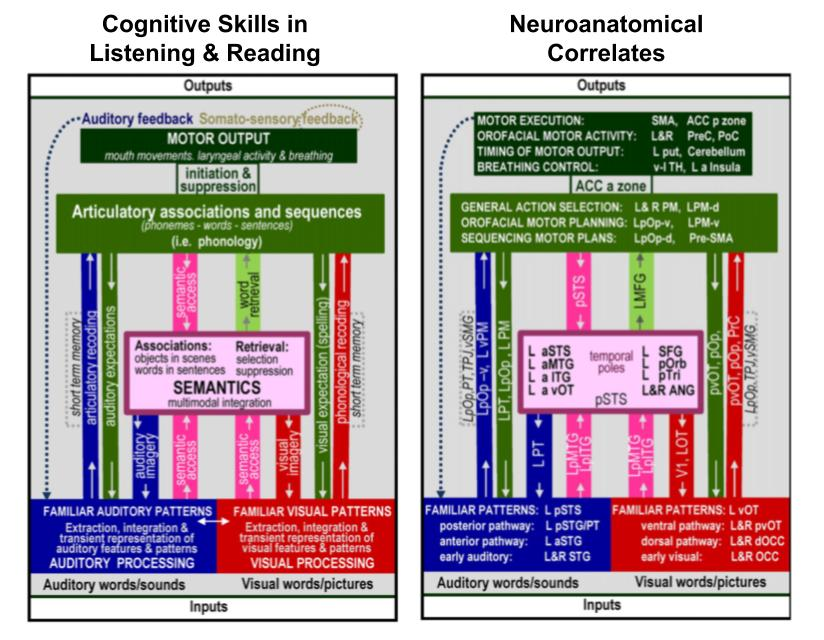
\includegraphics[height=3in]{images/ch2-price-language-models.jpg}
	\caption[Schematics of skills and brain areas used in reading.]{Models of reading typically focus on a common linguistic core that is responsible for comprehension and production of language. In this model, differences in modality affect input pathways to this core.}
	\label{fig:ch2-price-language-models}
\end{figure}

Despite the clear overlap between reading and listening, there is also evidence that the two skills are not directly equivalent. There is a subset of students who, despite adequate word decoding skills and vocabulary skills, struggle with reading comprehension\citep{Nation2010, Spencer2011}. From a neurobiological perspective, expected differences in primary visual (for reading) and primary auditory (for listening) represent the different input systems, with ventral occipito-temporal systems also activating \citep{Jobard2007}. However, differences in core language systems are also observed: additional activation in left posterior temporal and parietal areas in reading modality \citep{Constable2015}, as well increased bi-laterality especially in children \citep{Berl2010}. 

Most current cognitive models suggest that language comprehension requires the construction of a mental representation includes textual information and associated background knowledge, connected by some conscious and some unconscious executive processes \citep{Kendou2014}. The parallel model shown in Fig. \ref{fig:ch2-price-language-models} is linear: it moves from sensation to action. During comprehension, however, the relationship between areas is dynamic and constantly being re-evaluated. The roles of attention and executive systems are likely to play an important role. Thus, while there may be a core set of systems for manipulating and extracting meaning from language, it is likely that differences in modality would modulate these processes. 

The pioneering researcher Alvin Liberman suggested that reading, instead of being parallel to listening, is actually parasitic: it requires an 
textit{awareness} of the linguistic act that is not required in listening. Brain activation studies may not capture these differences: it could very well be the interactions of different functional systems that are changed, rather than the overall "engagement" of an individual brain area. Additionally, the fact that reading integrates in an additinoal modality could be a source of difference, especially in emerging readers. 

In this study, we pursue three hypothesized ways reading might differ from listening. These are not exclusive; one or more of them may be true. The overarching aim is to test whether reading is simply listening skills

\begin{itemize}
	\item Reading will require a greater "global" reorganization of resting-state networks than listening. This network will also be more highly integrated than that of listening. 
	\item Reading will reduce the modularity within the sensory system of interest. That is, visual areas will become less internally connected during reading, while auditory areas will be less internally connected during listening.
	\item Reading will make greater demands on attention systems than listening. That is, areas in the frontal and attention systems will be activated to a greater degree during reading than listening.
\end{itemize}

First, we validate modularity and participation coefficient metrics using univariate data, and test that language induces greater global integration, especially in higher-order networks (executive + default mode) compared to resting and attention baselines. Second, we test three hypotheses about how interactions between brain networks might differ from speech. Finally, we investigate whether these interactions change with experience, testing whether the reading and listening systems "merge" into a unified system or whether differences between reading and listening persist across development.


\section{Methods}

The following methods detail the current study's protocol and analytical approach. Many of these methods will be used in future studies and are explained in detail here. 

\subsection{Participants}

Participants for the first study were drawn from the fourth wave of a larger, longitudinal study investigating the neurobiological bases of reading comprehension. 52 children completed scans for the current study and a subset of these met the motion and attention thresholds described below. See Table \ref{table:ch2-participants} for demographics. 

All participants were native English speakers with normal hearing and normal or corrected vision, and no history of major psychiatric illness or traumatic brain injury/epilepsy. Subjects had no history of a developmental disability or contra-indication to MRI.  Each participant gave written consent at the beginning of the study, with procedures carried out in accordance with Vanderbilt University’s Institutional Review Board.

\begin{table}
	\renewcommand{\tabcolsep}{0.09cm}
	\centering
	\begin{tabular}{lc}
\toprule 
Measure & Subjects \\ 
\midrule 
No. Participants				& 42 \\ 
No. Scan Runs					& 164 \\ 
Gender  						& 25 F \\ 
Age at Scan 					& 10.5 (0.3)  \\ 
WASI Full-Scale IQ  			& 111.0 (16.2) \\ 
TOWRE - Total Word Efficiency 	& 104.6 (18.5) \\ 
\bottomrule 
\end{tabular}
	\caption[Participant demographics for Study 1.]
	\label{table:ch2-participants}
\end{table}


\subsection{Functional MRI Task}

We designed an fMRI task in which participants either read or listened to a passage of text. The passage was split into two paragraphs and interspersed with a simple attention task. At the end of the task, there was an approximately three minute long resting-state block. Across runs, conditions were presented in the same order, although durations varied slightly. Condition order was: comprehension block (paragraph 1), sensory baseline (set 1), comprehension block (paragraph 2), sensory baseline, and resting baseline. See Fig. \ref{fig:ch2-task-design} for a schematic.

\begin{figure}[t]
	\centering
	\includegraphics[height=3in]{images/ch2-eprime-recall.png}
	\caption[Schematic of the reading comprehension task.]
	\label{fig:ch2-task-design}
\end{figure}

To create a more naturalistic reading experience than single word presentation \citep{Rayner1986}, passages were presented in syntactic phrases ranging from 1-7 words in length. The interval between each stimulus was jittered to allow for event-related analyses (range: 275 – 4000 ms), although these effects were not examined here.

The sensory baseline condition was altered according to modality. For the reading runs, three non-alphanumeric symbols were displayed horizontally (two types), and their presentation time was matched to the passage phrases. Spacing between symbols was randomly alternated to replicate the variable phrase lengths in the passage condition. For the listening runs, three tones (two frequencies) were played in sequence, with a new set of tones beginning at the same intervals as the corresponding passage presentation. 

To monitor attention, 4 to 8 percent of the stimuli within each passage or attention block were randomly repeated on two consecutive screens.  Participants pressed a button with their right thumb when they detected a repeated phrase, symbol or tone configuration. Additionally, at the conclusion of each passage, a picture was presented on the screen, and subjects were asked to identify whether the picture had any relationship to the passage (e.g., a picture of a mushroom for a passage about fungi). 

To assess performance, we analyzed three measures: in-scanner attention, in-scanner comprehension, and post-scan recall. To assess attention, we calculated the $D`$ statistic ($Z(true\ positive) - Z(false\ positive)$) for the "repeated stimulus" task. The in-scanner comprehension measure was the number (0,1,2) of questions correclty answered. To assess recall, each child was asked to recite as much of the passage as they could remember, and their answers were mapped to actual phrases present in the chapter. Individual scan runs with a $D`$ value less than 2 were excluded from analysis.

In total, there were 4 passages (2 listening, 2 reading), each leveled to a 3\textsuperscript{rd} grade difficulty and balanced on word measures such as concreteness and cohesiveness.  All subjects were trained on the task in a mock scanner prior to the actual scan. 


\subsection{MRI acquisition}

Imaging was performed on a Philips Achieva 3T MR scanner with a 32-channel head coil. Functional images were acquired using a gradient echo planar imaging sequence with 40 (3 mm thick) slices with no gap. Each run of the task (up to four) consisted of 250 volumes. Slices were parallel to the anterior-posterior commissure plane. Imaging parameters for functional images included: TE = 30 ms; FOV = 240 x 240 x 120 mm\textsuperscript{3}; flip angle = 75\degree; TR = 2200 ms; and 3 mm\textsuperscript{3} isotropic voxels.

\subsection{Activation analyses}

Whole-brain fMRI analyses were performed using tools from the FMRIB Software Library (version 5.0.9). For each session, the following pre-processing steps were performed:  slice-time correction, motion correction to the initial fMRI volume, high-pass filtering at 0.08 Hz, boundary-based registration to the subject's structural image, and normalization to 2 mm MNI 152 standard space. To mitigate the effects of motion on our analyses, we regressed out 6 continuous motion parameters and scrubbed out outlier volumes. We defined an outlier volume as any in which the root-mean-square framewise displacement exceeded 0.7 mm. Because head motion can be a major confound for connectivity analyses, we removed scan runs where more than 10 percent of the fMRI volumes were outliers.

All task conditions were convolved with the double-gamma hemodynamic response function to generate design matrices for each fMRI run. Two first-level contrasts were of interest: the main effect of passage comprehension (“pass vs. rest), and the contrast of passage comprehension vs. the sensory baseline ("pass vs. attn."). Repeated stimuli and the picture comprehension task were modelled out.

Modality effects (Shared Effect of Listening and Reading, Contrast of Listening and Reading) were estimated at the subject-level using fixed effects analysis. These were carried over into group-level analyses using non-parametric methods implemented in FSL’s \textit{randomise} tool with threshold-free cluster enhancement. For each group-level analysis, we performed 10,000 permutations and report results with \textit{p} \textless 0.05. 

\subsection{Connectome analyses}

To investigate whole-brain patterns of connectivity without biasing our results towards our task, we selected 264 nodes \textit{a priori} whose connectivity properties have been extensively analyzed \citep{Power2011}. This node set samples the entire brain and are involved in a diversity of cognitive tasks. Each node was assigned to one of 13 RSNs based on previous literature \citep{Power2013}. Approximately 10 percent of the nodes did not have a stable assignment in the original paper; for the present analyses, these nodes were excluded from graph theory calculations. A description of the 13 networks, their size, and their overlap with the 2011 Yeo parcellation is provided in \ref{table:ch2-power-nodes}. 

\begin{table}
	\renewcommand{\tabcolsep}{0.09cm}
	\centering
	\begin{tabular}{lcc}
\toprule 
Suggested RSN & Abbreviation & Nodes \\ 
\midrule 
\textit{Sensory} & & \\
	\hspace{3pt}Auditory  			&  AUD & 13 \\ 
	\hspace{3pt}Somatomotor (Hand)	&  SOH & 30 \\
	\hspace{3pt}Somatomotor (Mouth)	&  SOM & 5 \\
	\hspace{3pt}Visual	 			&  VIS & 31 \\ 
\textit{Attention} & & \\
	\hspace{3pt}Dorsal attention  	&  DAN & 11	\\ 
	\hspace{3pt}Salience		  	&  SAL & 18 \\ 
	\hspace{3pt}Ventral attention  	&  VAN & 9 \\ 
\textit{Executive / Associative} & & \\
	\hspace{3pt}Cingulo-opercular 	& CON & 14 \\ 
	\hspace{3pt}Default mode		& DMN & 58 \\
	\hspace{3pt}Fronto-parietal  	& FPN & 25 \\ 
	\hspace{3pt}Memory retrieval	& MEM & 5 \\
\textit{Other} & & \\
	\hspace{3pt}Cerebellar			& CER & 4  \\
	\hspace{3pt}Subcortical			& SUB & 13 \\
	\hspace{3pt}Not assigned 		& UNC & 28 \\ 
\bottomrule 
\end{tabular}
	\caption{Networks used in connectivity analyses.}
	\label{table:ch2-power-nodes}
\end{table}

Network estimation was performed in the \textit{Conn: Functional Connectivity Toolbox} (version 17f) \citep{Nieto-castanon}. For each scan run, the BOLD activity at each node was denoised using the anatomical CompCorr method, which regresses out background noise from white matter and cerebrospinal fluid tissue. We also regressed out 12 continuous measures of motion were also included, all outlier timepoints, and the effect of all task conditions ("pass", "attn", "rest"). The timeseries was then high-pass filtered at 0.01 Hz.

Whole-brain connectomes for each condition were created by estimating the functional connectivity between each node using a weighted general linear model. For connection-level analyses, these values were compared directly across subjects and conditions. For graph theory analyses, the array of all node connections was thresholded to keep the top 5 percent of connections, resulting in a much sparser representation. This threshold was also tested at ranges from 2 percent to 10 percent.

The metrics of interest were network \textit{modularity} and \textit{participation coefficient}. Modularity is high in networks where nodes within the same RSN are highly connected to each other but not elsewhere. The participation coefficient, on the other hand, is high when many nodes are connected to several different RSNs. Both of these metrics relate to the integration of information between RSNs. These properties, and their changes within our task, were investigated at the level of connectomes, RSNs and nodes. 


\section{Results}

\subsection{Behavioral results}

42 subjects (142 scan runs) met the attention and motion criteria to be included in the analysis. (10 subjects and 61 individual scan runs were filtered out.) Attention and comprehension measures were not related to modality of stimulus presentation (see Figs. \ref{fig:ch2-eprime-recall} and \ref{fig:ch2-eprime-comprehension}). There was a trend towards difference in median FDRMS between scan modalities (paired t-test, $t = 1.94$, $p = 0.059$), so we also replicated analyses with a stricter motion threshold (no more than 10 percent outliers in a scan run), and analysis results were generally consistent.

\begin{figure}[t]
	\centering
	\includegraphics[height=3in]{ch2-eprime-recall}
    \caption[Out-of-scanner pasage recall was unrelated to modality.]{}
	\label{fig:ch2-eprime-recall}
\end{figure}

\begin{figure}[t]
	\centering
	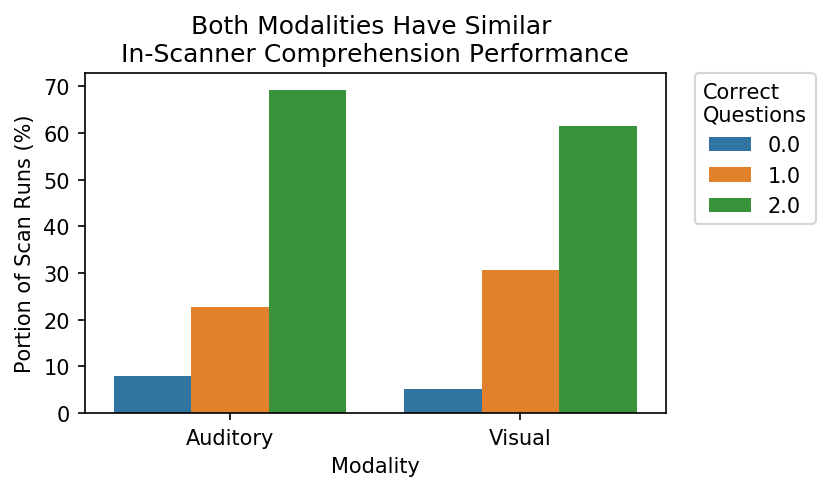
\includegraphics[height=3in]{ch2-eprime-comprehension}
    \caption[In-scanner comprehension performance did not differ by modality.]{}
	\label{fig:ch2-eprime-comprehension}
\end{figure}

\subsection{Activation results}

A range of language-related areas were activated for both reading and listening comprehension (Fig. \ref{fig:ch2-passages-activation-attn}). Compared to the corresponding sensory baselines, activation spanned the inferior frontal gyrus, angular gyrus, premotor cortex, middle temporal gyrus and the superior frontal gyrus. Activation patterns were robustly present on both hemispheres, but had greater intensity and extent on the left hemisphere. 

\begin{figure}[t]
	\centering
	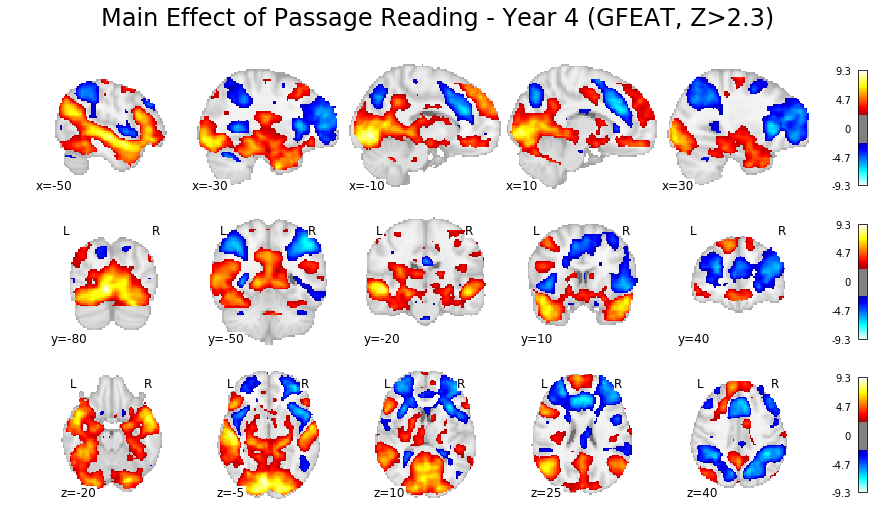
\includegraphics[height=3in]{ch2-passages-activation-attn}
    \caption[There is significant overlap between the areas used in listening and reading.]{A widespread set of brain areas are utilized during listening and reading, including auditory, default mode and attention areas.}
	\label{fig:ch2-passages-activation-attn}
\end{figure}

Differences related to modality fell into three categories: sensory processing areas, including the insula, superior temporal gyrus, and secondary visual processing areas; and hetero-modal association areas, most notably the inferior frontal gyrus and angular gyrus; and somato-motor regions, including the premotor cortex and lateral geniculate nucleus of the thalamus (Figure 2). Areas showing greater activation in listening were focused on primary auditory cortex and the dorsal attention network. 

\begin{figure}[!b]
	\centering
	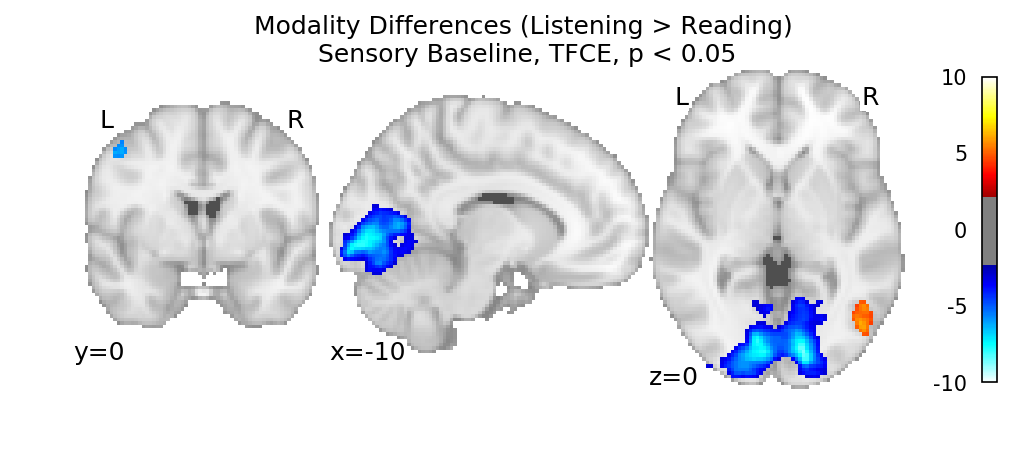
\includegraphics[height=3in]{ch2-modality-differences-attn}
    \caption[Modality differences center on primary sensory and integration areas.]{Modality differences center on primary sensory and integration areas.}
	\label{fig:ch2-modality-differences-attn}
\end{figure}

Overall, there was a high degree of similarity between the areas that were activated in reading and in listening, reflecting the common language core. When the statistics for each node in the connectome were plotted against each other, there was a very high correlation coefficient ($r = ___$), as seen in Fig. \ref{fig:ch2-listening-reading-connectome-activations}.

\begin{figure}[t]
	\centering
	\includegraphics[height=3in]{ch2-listening-reading-connectome-activations}
    \caption[There is significant overlap between the areas used in listening and reading.]{A widespread set of brain areas are utilized during listening and reading, including auditory, default mode and attention areas.}
	\label{fig:ch2-listening-reading-connectome-activations}
\end{figure}


\subsection{Connectome results}

Relative to rest, both listening and reading reduced the global modularity and increased the participation coefficient (Fig. \ref{fig:ch2-comprehension-graph-theory}. Compared to the baseline attention task, there were  trends towards an increased participation coefficient, but they were not significant. 

\begin{figure}[t]
	\centering
	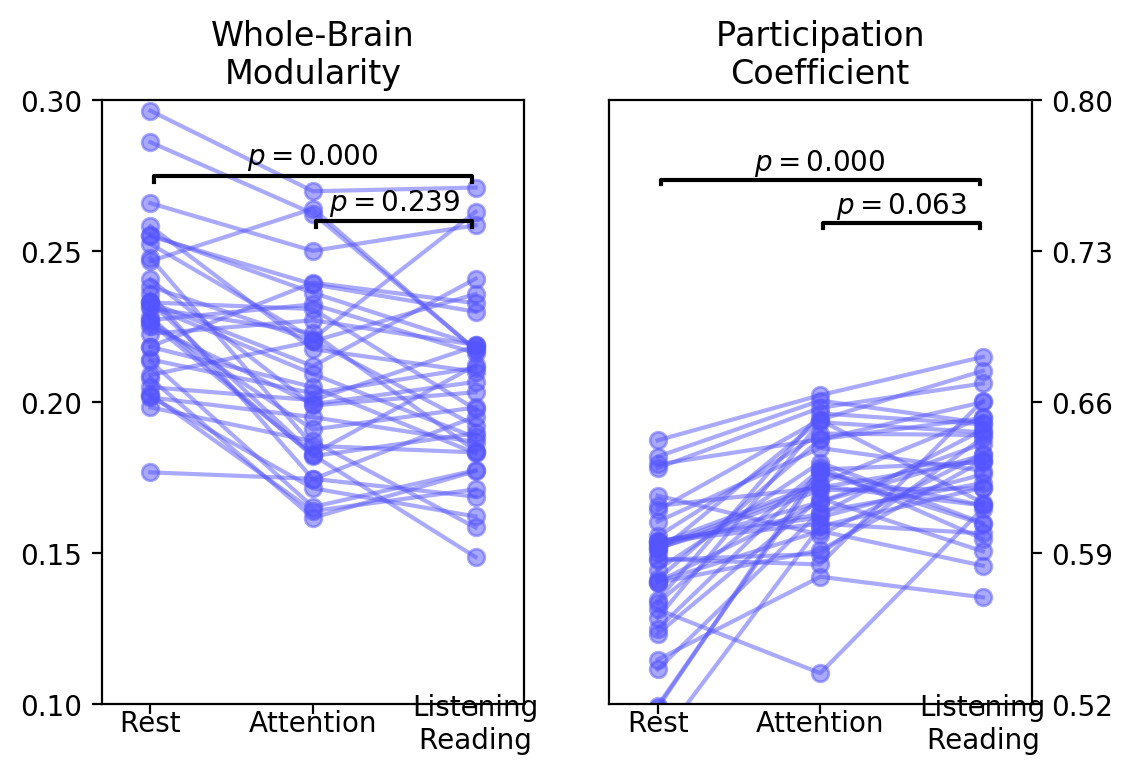
\includegraphics[height=3in]{ch2-comprehension-graph-theory}
    \caption[Language induces more integrated global network architecture.]{}
	\label{fig:ch2-comprehension-graph-theory}
\end{figure}

Comparing listening to reading showed that reading induced a more integrated network architecture than listening, both in terms of reduced modularity and increased participation coefficient (Fig. \ref{fig:ch2-modality-graph-theory}).  

\begin{figure}[t]
	\centering
	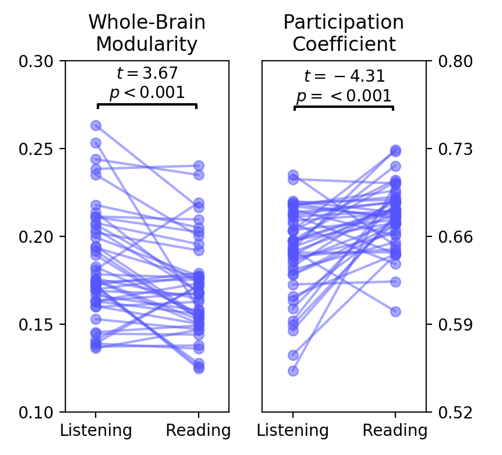
\includegraphics[height=3in]{ch2-modality-graph-theory}
    \caption[Reading is more integrated than listening.]{}
	\label{fig:ch2-modality-graph-theory}
\end{figure}

Summarizing changes in connectivity at the network level provides additional insight. When comparing comprehension differences to rest, for example, we can see that globally connectivity increases (Fig. \ref{fig:ch2-comprehension-reorganization}. During rest, however, there is increased connectivity within default mode network and visual networks.

\begin{figure}[t]
	\centering
	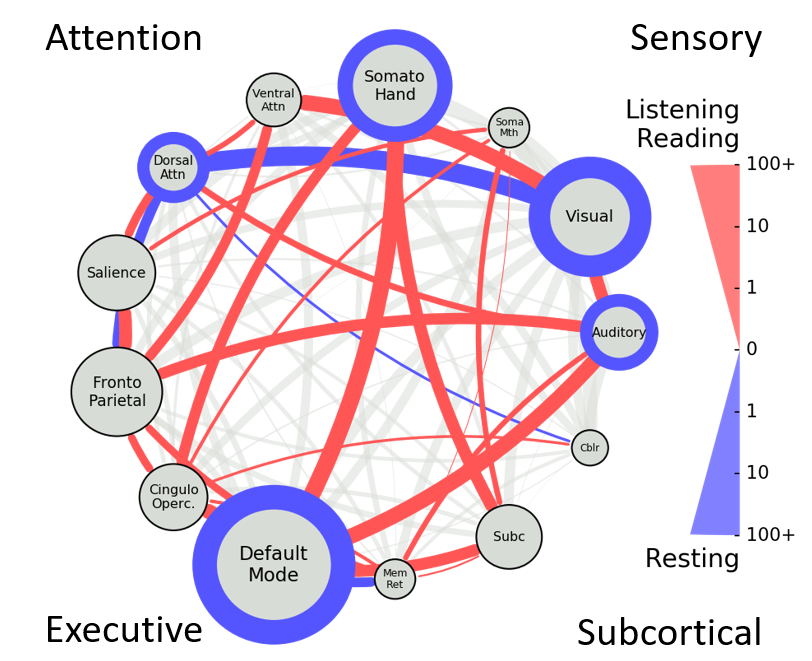
\includegraphics[height=3in]{ch2-comprehension-reorganization}
    \caption[Language increases between-network connectivity.]{}
	\label{fig:ch2-comprehension-reorganization}
\end{figure}

Summarizing changes in connectivity at the network level provides additional insight. When comparing comprehension differences to rest, for example, we can see that globally connectivity increases (Fig. \ref{fig:ch2-modality-reorganization}. During rest, however, there is increased connectivity within default mode network and visual networks.

\begin{figure}[t]
	\centering
	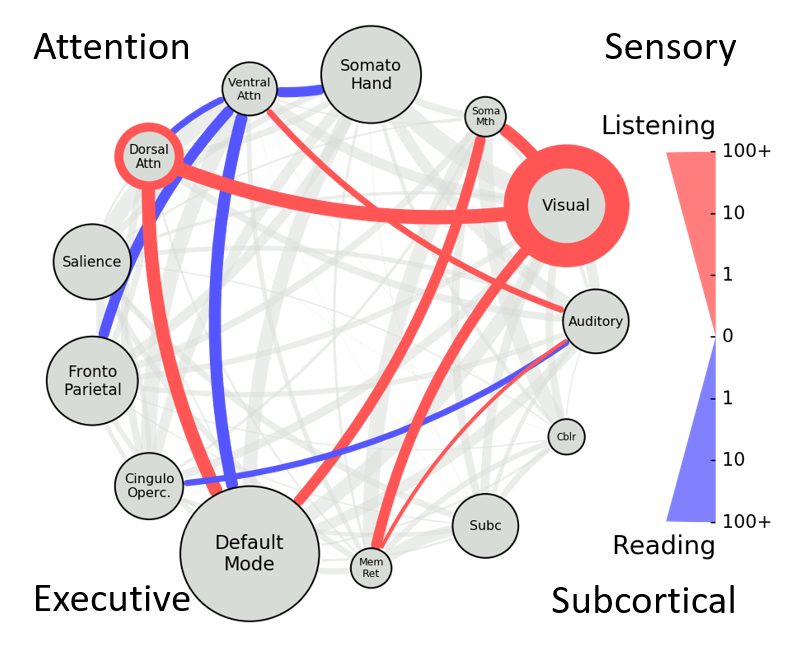
\includegraphics[height=3in]{ch2-modality-reorganization}
    \caption[Reading decreases connectivity within visual and dorsal attention networks.]{}
	\label{fig:ch2-modality-reorganization}
\end{figure}


\section{Discussion}

This study pushes further than previous studies have by investigating differences between reading and listening in terms of their activation of individual areas or the distribution of activity across the brain. We employ closely matched texts, large sample size, longitudinal sampling, and behavioral covariates. Comprehending extended text requires more than just sensory and linguistic processes. It also requires executive processes such as attention, working memory and inference. Since comprehension is a "whole-brain" activity, we here look at the reorganization of resting-state networks - to see how attention, executive and sensory systems are interacting during reading.

We tested three hypotheses related to global reorganization, sensory system changes, and interactions between executive and attention systems and sensory systems.

These modality-specific influences on behavior and brain activity may arise from a few different sources: subject, linguistic and innate differences. 

There are also differences in what is encoded in speech and text. The reading sciences pioneer Alvin Liberman noted that "speech is a complex code, while reading is a simple cipher" \cite{Mattingly1972}. Speech contains overt clues about the speaker, such as tone and prosody, and these can convey additional non-linguistic meaning for the listener. Reading, on the other hand, might be considered a more purely linguistic act, especially with computer-printed text. Reading may thus allow more room for self-generated situation models and more independent direction of thought. Furthermore, modality-specific aspects of the stimulus may influence the overall comprehension process; reading requires a level of spatial awareness -where one is at on a page, what happened in preceding paragraphs – and allows for the re-treading of information. Listening, meanwhile, requires the extraction of input from competing noises and sometimes the tracking of changing volume. 

People speak differently than they write. Reading often relies on more complicated syntax, and even for skilled readers, longer words and sentences can strain executive systems more than they might if being spoken to. Although these properties are often controlled for in scientific studies, they represent a major difference between “natural” reading and listening. Because of these differences, reading may place a greater load on executive function skills. Executive functions such as working memory and planning and organizing may be particularly important for reading \citep{Cain}.  

The last set of differences is particularly interesting because knowing how the differences in reading interact with these modality differences. Reading is a learned skill with may component processes. It requires thousands of hours of experience to master and entails a reorganization of cortical resources. Environmental and biological factors thus exert a greater influence on an individual’s reading proficiency than they might on more intrinsic processes such as speech comprehension. This is particularly dramatic in individuals with dyslexia, who have persistent difficulty with reading. Children with dyslexia exhibit less activation in reading-related areas compared to typically developing children \citep{Pugh2000}, but greater activation in right hemisphere homologues, suggesting that lateralization and activation of the reading circuit are associated with better reading. Development period also has an effect, with children exhibiting less activation in frontal areas but more in posterior areas, possibly reflecting a shift in “resource load” from uni-modal to supramodal areas \citep{Berl2010}. This shift may not be necessary in listening, or occur much earlier. Thus, with increasing expertise and development, there may be a “shift” from relying on fusiform processing areas. towards using multi-modal areas more like speech \citep{Monzalvo}. 

This interaction between reading activation and individual differences in maturity and reading skill will be the subject of the next chapter.